\title{Report on \\ Model Development for Fossil Fuel Divestment}
\author{Jakob J. Kolb \\ Potsdam Institute for Climate Impact Research}

\maketitle

\section{Model Development} 

Previous studies \cite{Ans2013} suggest that feedback through supply-demand price mechanisms will have only limited impact on fossil fuel companies. This is due to the fact, that only approximately 15 \% of investors invest subject to socially responsible guidelines \cite{SIF2014Report} and that divested holdings are, especially in liquid markets, very likely to quickly find their way to less responsible investors. \\
Also, as long as the physical capital relying on fossil fuels already exists, economic reasoning follows that it will be used as long as variable costs are covered.
Therefore, a general economic shift from dirty to clean technology can only arise from changes in investment in physical capital or from political imperative mandated by a (qualified) majority. Therefore, I consider a model focussing on savings and investment decisions appropriate to investigate the possible dynamics of an economic transition towards fossil resource independent technologies.\\
In the following I propose a preliminary scheme of such a model.

\begin{figure}[h]
	\centering
	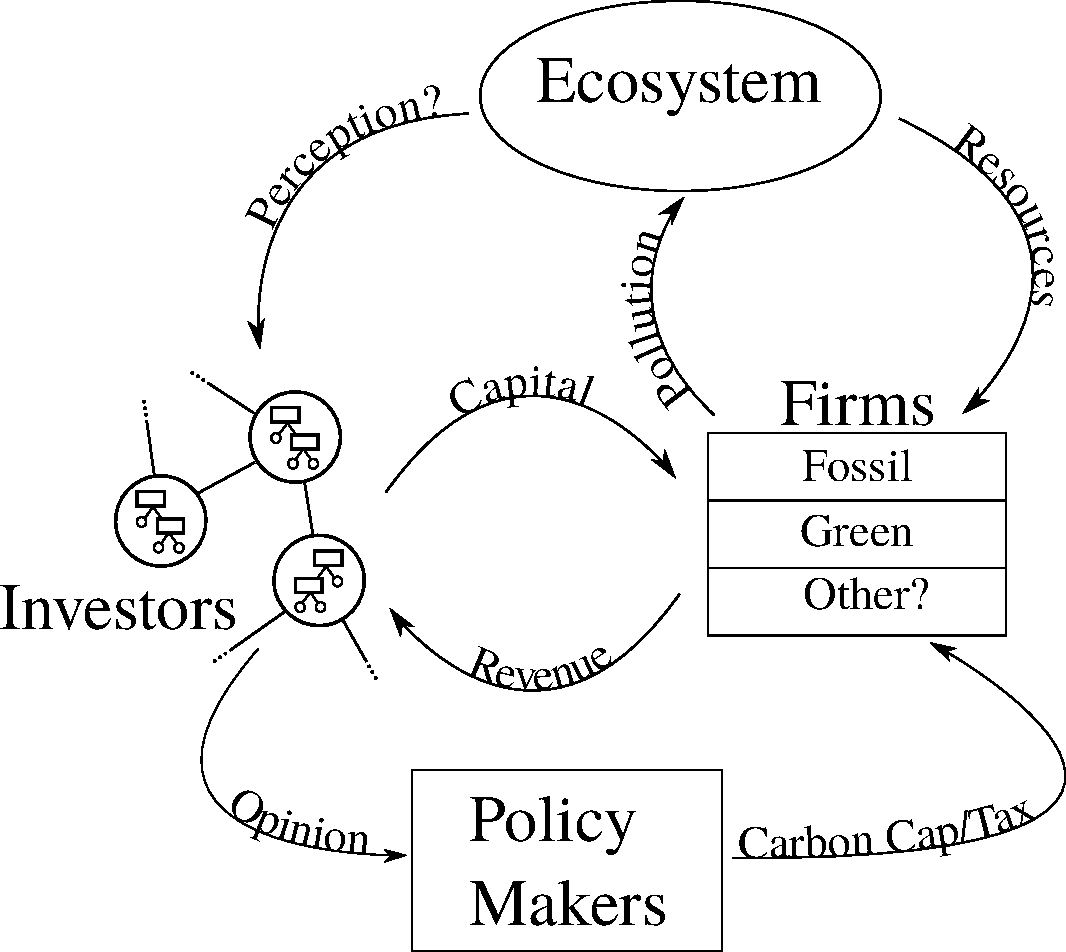
\includegraphics[width =.7 \textwidth]{figures/Model_Scheme.pdf}
	\caption{Schematic sketch of the model including four major components: Households, Firms (grouped by sector), Ecosystem and optional Policy makers.}
	\label{fig:model}
\end{figure}

\subsection{Economic Model}


\subsubsection{Sectors}

Production is assumed to take place in two sectors. One sector $(d)$ employs a dirty technology depending on fossil resources, the other sector $(c)$ employs a clean technology relying on renewable resources. The physical capital is assumed to be bound to this technology, e.g.\ there are two separate capital stocks $K_d$ and $K_c$. Both sectors use capital $K_j$ and labor $P_j$ as input factors. The dirty sector additionally uses a fossil resource $R$ whereas the clean sector additionally relies on developing knowledge about the relevant technologies:
\begin{align}
	Y_d = F_d(K_d,P_d,R) \\
	Y_c = F_c(K_c,P_c,C)
	\label{eq:production}
\end{align}

\subsubsection{Production Functions}
For the inputs of labor $P$ and capital $K_j$, a Cobb-Douglas type production function is assumed. For the fossil resource input, a Leontief type production function is assumed, since energy (coming from the fossil resource) can hardly be substituted in general. The knowledge about green technologies is assumed to be capital augmenting. This results in the following production functions:
\begin{align}
	Y_c &= b_c (C^\xi K_c)^{\kappa_c} P_c^{\pi_c} \\
	Y_d &= {\rm min}(b_d K_d^{\kappa_d} P_d ^{\pi_d}, e R)
\end{align}
where $e$ is the fossil resource efficiency.

\subsubsection{Resource extraction}
The total cost flow for fossil resource extraction $c_R$ (exploration and exploitation) is assumed to scale with $R^{\varepsilon}$.
\begin{equation}
	c_R = b_R R_d^{\varepsilon}
	\label{resource_extraction_cost}
\end{equation}
The factor $b_R$ represents the effort necessary to locate and develop fossil resources. It is presumably depending on the remaining Fossil resource $G$ stock and increasing as the remaining resource decreases. Further, it is assumed to diverge, as $G$ approaches zero. Also, efficient allocation of resource is assumed, e.g.\ there are no idle resources in the dirty sector. Consequently,
\begin{equation}
	Y_d = b_d K_d^{\kappa_d} P_d^{\pi_d} = e R.
	\label{efficient_resource_extraction}
\end{equation}
\subsection{Learning in the clean sector}
\label{learning}
The stock of knowledge about clean technologies $C$ that augment clean capital $K_c$ in the clean sector is assumed to grow through learning by doing, e.g.\ output of the clean sector leads to increase in knowledge. The knowledge stock is also assumed to deteriorate with a fixed rate due to staff turnover, depreciation of machines, or simply forgetting tacit knowledge about the technology. Therefore, the knowledge stock develops as
\begin{equation}
	\dot{C} = Y_c - \zeta C
	\label{knowledge_stock}
\end{equation}
\subsubsection{Capital Rent and Wages}
We assume perfect labor mobility, resulting in equal wages in both sectors. We also assume that on the labor and capital market, sectors are price takers, e.g.\ that wages and capital rental rates are equal to the marginal increase in output per unit input. (Note that in the dirty sector, increase in input factors also result in increasing resource costs $c_R$):
For capital rent and wages, this results in the following conditions:
\begin{align}
	w &= \frac{\partial Y_c}{\partial P_c} = \frac{\partial Y_d}{\partial P_d} - \frac{\partial c_R}{\partial P_d}\\
	r_c &= \frac{\partial Y_c}{\partial K_c}\\
	r_d &= \frac{\partial Y_d}{\partial K_d} - \frac{\partial c_R}{\partial K_d}
\end{align}

\subsection{Households}
In contrast to common economic growth models, I abject the notion of one representative household. We rather assume heterogeneous households, each with their own income and independent in their savings decisions. This allows to investigate certain features, that consider crucial with respect to my research question.
\begin{itemize}
	\item Changing norms amongst households with respect to what is important to consider in savings decisions,
	\item Network effects in this norm/opinion dynamics that are driven by heterogeneity amongst individuals.
\end{itemize}

\subsubsection{Income and savings}
Households denoted with the Index $i$, $i \in [1, \dots N]$ are are owners of capital $K_j$ as well as suppliers of labor $P_j$. For simplicity, I assume that each household has the same number of members, each supplying one unit of labor per unit of time $t$. The income of the household comes from capital returns and labor income:
\begin{equation}
	I_i = \sum_j r_j K^{(j)}_{i} + w\frac{P}{N}
	\label{eq:household_income}
\end{equation}
Households are assumed to save at a fixed rate $s$ and reinvest their savings in one of the two types of capital ($K_c$ and $K_d$) available. \\
\textit{For now, capital investment is considered irretrievable and capital can not be traded. Empirical data suggests a more or less constant savings rate of 23 \%} \\

\subsubsection{Savings investment - decision making}
Households have to decide in which of the two capital goods they want to invest their savings. Decision makers are assumed to have no knowledge of the future, e.g.\ they make decisions based solely upon information about the past and present. Possible sources of information are the economic system and other households as so far as they interact with them.\\
\textbf{Possible decision cues are:}
\begin{itemize}
	\item the capital rent for the two savings options $r_c$ and $r_d$,
	\item the trend in these capital rents $\dot{r}_c$ and $\dot{r}_d$,
	\item the option the majority of the households neighbors opt for,
	\item the morale of investing in clean technology due to negative externalities (that are not factored in in the returns)
\end{itemize}
Households are assumed to use bounded rational reasoning to infer investment decisions from these cues. Considering different decision heuristics for the given decision environment (binary decision with a number of cues for each option) the \textit{Take The Best Heuristic} seems to be a suitable candidate. \\
In general, Fast and Frugal Heuristics are described in terms of three building blocks; one for information search, one for stopping information search and one for evaluating the available information and drawing a conclusion from it.
Take the Best has the following building blocks: 1) Search through cues in a predefined order, 2) stop as soon as one cue discriminates between the two options, 3) chose the option with the preferable value on the discriminating cue. \\
This requires a so called \textit{cue order} e.g.\ a hierarchy of validity for the pieces of information that are considered relevant for the decision. \\
Research on perception and decision making in psychology where the concept of Fast and Frugal heuristics was developed usually considers inferential decisions (since they have true and false outcomes and can therefore be benchmarked and evaluated statistically).\\
Nevertheless, Heuristic decision making is a reasonable tool for preferential decisions as well. Although in this context the interpretation of cue orders would be different - namely, they would rather be considered as norms or underlying preferences that apply to the context of the decision. \\
The case of savings decisions that is considered in this model poses an intermediate case for a number of reasons. First, there is no immediate feedback on savings decisions, since the return on investment depends on the future development of the economic system which in return depends on the savings decision of all the other households and second, we assume that households do not only consider financial but also moral grounds for their savings decisions. Nevertheless, some strategies are suspected to have more profitable long term results then others.\\
Also, we assume, that imitation of peers is not only a valuable strategy in many situations but also a value in its own - especially if the question is to some extend one of morale. 
Therefore, in the context of this model, I interpret the cue order $O$ of the decision heuristics as preferences/opinions resulting from a conceptual social dynamic. \\

\textit{The given framework might as well be used to test other strategies for decision making such as tallying or pure social learning similar to the approach taken by Barkoczi \cite{Barkoczi2013a}, \cite{Barkoczi2016}}

\subsubsection{Opinion formation and social dynamics}
Technically, this means that households are connected by a social network. Households are nodes, connections are links, links form an unweighted, undirected network that is represented by an adjacency matrix $A_{kl}$.
The dynamics of and on the network follow a slightly modified \textit{adaptive voter process}:
The activity of households is given by a Poisson process e.g.\ the waiting times $\Delta t$ for a household to become active are distributed as
\begin{equation}
	p(\Delta t) = \frac{1}{\tau} \exp\left[-\frac{\Delta t}{\tau} \right].
	\label{waiting_time_distribution}
\end{equation}
When a household becomes active, it does the following:
\begin{itemize}
	\item it chooses one of his neighbors to compare itself to,
	\item if their preferences differ, one of two things happen:
	\item with probability $\varphi$ the selected household $k$ cuts
		the link to the selected neighbor $l$ and establishes a new
		link to a random neighbor with the same preferences
	\item with probability $1-\varphi$ they compare a fitness parameter $W_k$
		which is household income in our case given by the households Income $I_i$: 

		\begin{equation}
			W_i = I_i = \sum_j r_j K^{(j)}_{i} + w\frac{P}{N}.
			\label{eq:fitness}
		\end{equation}

		if if the neighbors fitness is higher, the active household $k$
		adopts the neighbor $k$'s preferences $(S_k \rightarrow S_l)$ with a sigmoid shaped 
		probability:
		\begin{equation}
			P(S_k \rightarrow S_j) = 1/2 (\tanh(I_k - I_l)-1)
			\label{imitation_probability}
		\end{equation}
\end{itemize}

This process has two kinds of stable states. States in which all nodes have the same opinion and states in which the network separated to different fragments of nodes holding the same opinion. In our case, this is somewhat pathological, since it allows for groups of households to persistently invest in stranded assets. \\
This can be avoided by introducing noise in form of a small fraction of imitation and rewiring events that lead to either random selection of one of the possible cue orders or randomly rewiring to a household disregarding its opinions.

\subsection{Ecosystem}
Ecosystem is the source of resources and the sink for pollution. Minimal implementation would be a fixed carbon stock that is exploited by the fossil fuel sector. Optionally one could implement some sort of climate impact as a consequence of pollution.

In the case under study, we assume a non renewable geological carbon stock $G$, that is exploited by fossil resource uptake of the dirty sector:
\begin{equation}
	\dot{G} = -R
	\label{resource_dynamics}
\end{equation}
For the resource extraction efficiency $b_R$, we assume the following dependency on $G$:
\begin{equation}
	b_R = \tilde{b}_R \left( \frac{G_0}{G} \right)^{2}
	\label{extraction_efficiency}
\end{equation}


\subsection{Policy Makers}
\textit{Optional:} \\
Policy makers can implement some carbon tax or carbon cap on economy to incentivize green development. The implementation of such measure depends on the prevalence of opinions amongst voters (are investors a representative sample of voters?) and might be appropriately implemented by a Poisson distributed random variable.

\subsection{Variables}

\subsubsection{Dynamic Variables:}

\begin{table}[H]
	\centering
	\begin{tabular}{r|l}
		Variable & Description \\\hline
		$K^{(c)}_i(t)$ & clean investment of household $i$ \\
		$K^{(d)}_i(t)$ & dirty investment of household $i$ \\
		$G(t)$ & Geological carbon stock \\
		$A_{kl}(t)$ & Adjacency matrix \\
		$O_i(t)$ & opinion/cue order of household $i$ \\
		$x_i(t) \in [c,d]$ & investment decision of household $i$ 
	\end{tabular}
	\caption{Variables of the model with description.}
	\label{tab:independent_variables}
\end{table}
 
\subsubsection{Derived Variables}

\begin{table}[H]
	\centering
	\begin{tabular}{r|l}
		Variable & Description \\\hline
		$w(t)$   & Wage rate, \\
		$r_j(t)$ & Capital return rate in sector $j$, \\
		$c_R(t)$ & Fossil resource extraction cost, \\
		$b_R$	 & resource extraction `effort'\\
		$Y_j(t)$ & Output of sector, $j$ \\
		$P_j(t)$ & total labor employed in sector $j$, \\
		$K_j(t)$ & Total capital employed in sector $j$, \\
		$R(t)$ & Rate of resource uptake of dirty sector. \\
	\end{tabular}
	\caption{Variables of the model with description.}
	\label{tab:derived_variables}
 \end{table}

\subsection{Parameters}

\begin{table}[H]
	\centering
	\begin{tabular}{r|l}
		Parameter & Description \\\hline
		$\kappa_j$ & Capital elasticity in sector $j$ \\
		$\pi_j$ & Labor elasticity in sector $j$ \\
		$\rho$ & Fossil resource elasticity in dirty sector \\
		$b_j$ & total factor productivity in sector $j$ \\
		$\tilde{b}_R$ & resource uptake efficiency for fossil resource \\
		$P$ & Total population \\
		$s$ & savings rate \\
		$\delta $ & Capital depreciation rate \\
		$\tau$ & activity rate of households \\
		$\varphi$ & rewiring probability given an interaction event
	\end{tabular}
	\caption{Parameters of the model with description.}
	\label{tab:parameters}
\end{table}
 
\subsection{Dynamic equations}
To wrap up, the economic subsystem of the model can be described by the following ordinary differential equations:
\begin{align}
	\dot{K}_i^{(c)} &= s \delta(x_i - c) (r_c K_i^{(c)} + r_d K_i^{(d)} + w P_i) - \delta K_i^{(c)} \nonumber \\
	\dot{K}_i^{(d)} &= s \delta(x_i - d) (r_c K_i^{(c)} + r_d K_i^{(d)} + w P_i) - \delta K_i^{(d)} \nonumber \\
	\dot{P} &= \alpha P \nonumber \\
	\dot{G} &= - R 
\end{align}
that are subject to the following algebraic constraints:
\begin{align}
	P_c + P_d &= P \label{population} \\
	\frac{\partial Y_c}{\partial P_c} &= \frac{\partial Y_d}{\partial P_d} - \frac{\partial c_R}{\partial P_d} \label{wages} \\
	e R &= Y_d = b_d K_d ^{\kappa_d} P_d^{\pi_d} \label{resources}
\end{align}
and $r_c$, $r_d$ and $w$ are given by the respective marginal productivities:
\begin{equation}
	r_c = \frac{\partial Y_c}{\partial K_c}, \qquad r_d = \frac{\partial Y_d}{\partial K_d} - \frac{\partial c_R}{\partial K_d}, \qquad w = \frac{\partial Y_c}{\partial P_c} \label{wages_and_rents}
\end{equation} 


\section{Implementation} 

We assume equal labor elasticities in both sectors ($\pi_c = \pi_d$), linear resource extraction costs ($\varepsilon=1$) and no profits.

The conditions for labor shares and wages as well as optimal resource uptake pose algebraic constraints for the system of ordinary differential equations that describe the dynamics of the capital stocks $\dot{K}_i^{(j)}$, the resource stock $\dot{G}$ and the population growth $\dot{P}$

\subsection{Calculation of wages, resource uptake and capital rent}

To calculate labor shares $P_c$ and $P_d$ as well as wages in the two sectors, we use equations \eqref{wages} resulting in
\begin{align}
	w &= \frac{\partial Y_d}{\partial P_d} - \frac{\partial c_R}{\partial P_c} \nonumber \\
	&= \frac{\partial Y_d}{\partial P_d} - \frac{\partial c_R}{\partial R} \frac{\partial R}{\partial P_d} \nonumber = \frac{\partial Y_d}{\partial P_d} - \frac{\partial c_R}{\partial R} \frac{\partial}{\partial P_d} \frac{Y_d}{e} \nonumber \\
	&= \frac{\partial Y_d}{\partial P_d} - b_R \frac{\partial}{\partial P_d} \frac{Y_d}{e} = b_d K_d^{\kappa_d} \pi P_d^{\pi-1}\left( 1-\frac{b_R}{e} \right)
	\label{dirty_wages}
\end{align}
for the dirty sector and
\begin{equation}
	w = b_c K_c^{\kappa_c} \pi P_c^{\pi-1}
	\label{clean_wages}
\end{equation}
for the clean sector. Combining these results via equation \eqref{population} results in
\begin{equation}
	P = \left( \frac{w}{\pi} \right)^{\frac{1}{\pi-1}}\left( \left( b_c K_c^{\kappa_c} \right)^{\frac{1}{1-\pi}} + \left( b_d K_d^{\kappa_d} \left( 1 - \frac{b_R}{e} \right)^{\frac{1}{1-\pi}} \right) \right)
\end{equation}
substituting 
\begin{equation}
	X_c = (b_c K_c^{\kappa_c})^{\frac{1}{1-\pi}}, \qquad X_d = (b_d K_d^{\kappa_d})^{\frac{1}{1-\pi}}, \qquad X_R = \left( 1 - \frac{b_R}{e} \right)^{\frac{1}{1-\pi}}
	\label{substitutions}
\end{equation}
holds the following result for $w$:
\begin{equation}
	w = \pi P^{\pi-1}\left( X_c + X_d X_R \right)^{1-\pi}.
	\label{wage_result}
\end{equation}
Plugging this into equations \eqref{dirty_wages} and \eqref{clean_wages} results in 
\begin{align}
	P_c &= P \frac{X_c}{X_c + X_d X_R} \label{clean_labor} \\
	P_d &= P \frac{X_d X_R}{X_c + X_d X_R} \label{dirty_labor}
\end{align}
and plugging this into \eqref{resources} results in
\begin{equation}
	R = \frac{b_d}{e}K_d^{\kappa_d}P^{\pi}\left( \frac{X_d X_R}{X_c + X_d X_R} \right)^{\pi}.
	\label{R_result}
\end{equation}
Using the results for $P_c$ and $P_d$ together with equations \eqref{wages_and_rents}, the capital rental rates result in
\begin{align}
	r_c &= \frac{\kappa_c}{K_c}X_c P^{\pi}\left( X_c + X_d X_R \right)^{-\pi}, \label{r_c_result}\\
	r_d &= \frac{\kappa_d}{K_d}X_d X_R P^{\pi}\left( X_c + X_d X_R \right)^{-\pi}. \label{r_d_result}
\end{align}
It is also worth noting, that the assumption of zero profits, e.g.
\begin{align}
	Y_c &= w P_c + r_c K_c \nonumber \\
	Y_d &= w P_d + r_d K_d + c_R \nonumber
\end{align}
results in the following restraints for the capital and labor elasticities $\pi$, $\kappa_c$ and $\kappa_d$:
\begin{equation}
	\kappa_c = \kappa_d = 1-\pi.
	\label{elasticities_restriction}
\end{equation}
\textbf{Equations that are actually implemented are:}
\begin{subequations}
\begin{empheq}[box=\widefbox]{gather}
	X_c = (b_c K_c^{\kappa_c})^{\frac{1}{1-\pi}}, \qquad X_d = (b_d K_d^{\kappa_d})^{\frac{1}{1-\pi}}, \qquad X_R = \left( 1 - \frac{b_R}{e}\frac{G_0^2}{G^2} \right)^{\frac{1}{1-\pi}}, \\
	w = \pi P^{\pi-1}\left( X_c + X_d X_R \right)^{1-\pi}, \\
	r_c = \frac{\kappa_c}{K_c}X_c P^{\pi}\left( X_c + X_d X_R \right)^{-\pi}, \\
	r_d = \frac{\kappa_d}{K_d}X_d X_R P^{\pi}\left( X_c + X_d X_R \right)^{-\pi}, \\
	R = \frac{b_d}{e}K_d^{\kappa_d}P^{\pi}\left( \frac{X_d X_R}{X_c + X_d X_R} \right)^{\pi}, \\
	\dot{K}_i^{(c)} = s \delta(x_i - c) (r_c K_i^{(c)} + r_d K_i^{(d)} + w P_i) - \delta K_i^{(c)}, \\
	\dot{K}_i^{(d)} = s \delta(x_i - d) (r_c K_i^{(c)} + r_d K_i^{(d)} + w P_i) - \delta K_i^{(d)}, \\
	\dot{G} = - R, 
\end{empheq}
\end{subequations}
assuming that the timescale of the population growth is sufficiently slow to treat population $P$ as a parameter in the system.
\subsection{Opinion formation and decision making}
\label{sec:oppinion_formation_and_decision_making}
Households use the Take the Best heuristic to make investment decisions. This heuristic chooses between two options. Therefore, it sequentially evaluates cues (pieces of information), and as soon as one discriminates, it takes the option with the higher value on the discriminating cue. Possible cues in our model are:
\begin{itemize}
	\item[0] investment is dirty,
	\item[1] investment is clean,
	\item[2] Capital return rate $r_c$ and $r_d$,	
	\item[3] trend of capital return rates $\dot{r}_c$ and $\dot{r}_d$, interpolated from previous capital rents,
	\item[4] action observed in the majority of neighbors.
\end{itemize}
Preferences or opinions (I use the expressions synonymously in the context of this model) of the households are combinations of these cues without repetition. Investment decisions according to these preferences are updated immediately. \\
Since the number of possible combinations of these opinions is large ($38$) and consequently, to get statistically valid results one would need a very large number of households ($ ~ 10^2 \times 38$), which would be computationally expensive, we reduce the number of cue combinations to a set of presumably relevant `types':
\begin{itemize}
	\item [[2, 3]]: myopic investor,
	\item [[3, 2]]: trend sensitive investor,
	\item [[4, 2]]: myopic herder,
	\item [[4, 3]]: trend sensitive herder,
	\item [[4, 1]]: Green conformer,
	\item [[4, 0]]: Conservative conformer,
	\item [[1]]: `Gutmensch',
	\item [[0]]: Redneck
\end{itemize}
It is assumed, that these opinions that are the reasoning for individual decision making are spread amongst households in an opinion dynamics process. This opinion dynamics process is a variation of the adaptive voter model. The activity of households is governed by a poison process with mean waiting time $\tau$. If a households becomes active, it randomly chooses one of its neighbors to interact with and if they are of different opinion, there are two possible options:
\begin{itemize}
	\item [1)] with probability $\varphi$ the households cuts the link to its neighbor and connects to a random neighbor with the same opinion,
	\item [2)] with probability $1-\varphi$ they compare their income and with probability $P(x_k \rightarrow x_j)$ the household adopts the opinion of its neighbor.
\end{itemize}
The imitation probability monotonously increases with the income difference between the households: 

\begin{equation} 
	P(x_k \rightarrow x_j) = 1/2 ({\rm tanh}(I_k - I_l)-1).
	\label{primitive_imitation_probability}
\end{equation}

To eliminate pathological attractors of this dynamic (as mentioned earlier), a fraction $\varepsilon$ of the rewiring and imitation events are assumed to be random, e.g.\ leading to households making a new connection to another household uniformly at random and in disregard of his opinion or adopting a new opinion amongst the set of opinions that are possible in the system.

\newpage
\subsection{Limiting cases and timescales}
To estimate some parameters of the system, we analyze some limiting cases of the system and compare them with real world timescales. Such, we can set reasonable values to some parameters.
\subsubsection{Full on dirty economy}
Assuming, the fossil resources are very large, the dirty capital stock is significantly more profitable than the clean capital stock and subsequently all households decided to only invest in dirty capital. In this case we can treat the dirty sector isolated:
\begin{equation}
	\dot{K}_d = s I - \delta K_d, \quad I = w P + r_d K
	\label{eq:full_dirty_ca1}
\end{equation}
As we have found out before, $r_d$ is given by:
\begin{align}
	r &= \frac{\partial Y}{\partial K_d} - \frac{\partial c_R}{\partial K_d}, \quad c_R = b_R\left( \frac{G_1}{G} \right)^{2} R, \quad Y_d = eR, \\
	&\approx \left( 1-\frac{b_R}{e} \right)\frac{\partial Y_d}{\partial K_d},
	\label{eq:full_dirty_capital_rent}
\end{align}
and similarly for the wage $w$:
\begin{equation}
	w = \left( 1-\frac{b_R}{e} \right)\frac{\partial Y_d}{\partial P}.
	\label{eq:full_dirty_wage}
\end{equation}
So combining these, the income $I$ is equal to
\begin{equation}
	I = \left( 1-\frac{b_R}{e} \right)b_d (\kappa + \pi) P^{\pi} K_d^{\kappa}
	\label{eq_full_dirty_income}
\end{equation}
and using the fact that $\kappa + \pi = 1$ due to the fact, that there are no profits, the equation for capital accumulation \eqref{eq:full_dirty_ca1} reads
\begin{equation}
	\dot{K}_d = s\left( 1 - \frac{b_R}{e} \right) b_d P^{\pi} K_d^{\kappa} - \delta K_d
	\label{eq:full_dirty_ca2}
\end{equation}
This ordinary nonlinear differential equation can be solved by separation of variables.
\begin{equation}
	K_d (t) = \left( K_d^{*\ \pi} - C_1 e^{t/t_d^{*}} \right)^{\frac{1}{\pi}}
	\label{eq:dirty_capital_ac_solution}
\end{equation}
where the timescale for capital accumulation $t^*_d$ and the equilibrium dirty capital stock $K^*_d$ are
\begin{equation}
	t_d^{*} = \frac{1}{\pi \delta}, \qquad K_d^{*} = \left( \frac{s}{\delta}b_d P^{\pi}\left(1-\frac{b_R}{e}  \right) \right)^{\frac{1}{\pi}}.
	\label{eq:dirty_capital_equilibrium_values}
\end{equation}
Since the capital depreciation rate $\delta$ is (at least for infrastructure) around 5\% p.a.\ and estimates for the capital elasticity are around $\kappa_d=1/2$ (which we have also already assumed previously), the timescale for capital accumulation is $t^*_d \approx 40 y$. \\


\newpage

\subsubsection{Full clean economy}
\begin{wrapfigure}[16]{o}{.55 \textwidth}
	\vspace{-1.5 cm}
	\includegraphics[width = .9 \textwidth]{./figures/phasespace.pdf}
	\caption{Phase space plot of equations \eqref{eq:full_clean_ca} \label{phase_space_plot}}
\end{wrapfigure}
Along the same lines, we can treat the case of a full clean economy (assuming that the fossil resource is depleted, or the households have for some other reason decided to only invest in clean capital $K_c$). \\
In this case, the equations for capital and knowledge accumulation are
\begin{align}
	\dot{K}_c &= s b_c P^{\pi} (C^\xi K_c)^{\kappa} - \delta K_c \\
	\dot{C} &= b_c P^\pi (C^\xi K_c)^\kappa - \chi C
	\label{eq:full_clean_ca}
\end{align}
Assuming that capital and knowledge depreciate at equal rates, that $\kappa = \pi$ and no profits, the stationary points of the system are 
\begin{equation}
	(K_c^*, C^*) = (0,0), \left(s^{\frac{1}{1-\xi}}\left( \frac{b_cP^{\frac{1}{2}}}{\delta} \right)^{\frac{2}{1-\xi}}, s^{\frac{2-\xi}{1-\xi}}\left( \frac{b_cP^{\frac{1}{2}}}{\delta} \right)^{\frac{2}{1-\xi}}  \right)
	\label{stationary_points}
\end{equation}
where the first one is non hyperbolic and the second one is stable which can be seen in the phase space plot \ref{phase_space_plot} and the corresponding Jacobian
\begin{equation}
	J_{(K_c^*,C^*)} = 
		\begin{pmatrix}
			-\frac{1}{2}\delta & \frac{1}{2}\xi s \delta \\
			\frac{\delta}{2 s} & \delta \left( \frac{\xi}{2}-1 \right)
		\end{pmatrix}
	\label{eq:learning_jacobian}
\end{equation}
whose Eigenvalues are negative:
\begin{equation}
	\lambda_{1,2} = \frac{\delta}{2}(\xi-1), \quad -\delta
	\label{eq:learning_eigenvalues}
\end{equation}
The phase space plot \ref{phase_space_plot} also suggests that there is a trajectory that satisfies 
\begin{equation}
	\frac{K_c(t)}{C(t)} = \frac{K^*_c}{C^*}
\end{equation}
meaning, one has to find a solution to the following ode:
\begin{equation}
	\dot{K}_c = s^{1-\frac{\xi}{2}} b_C P_C^{\frac{1}{2}}K_C^{\frac{1}{2}(1-\xi)} - \delta K_C
	\label{eq:learning_trajectory_ode}
\end{equation}
which can be done by means of separation of variables, resulting in
\begin{equation}
	K_c(t) = \left( s^{1-\frac{\xi}{2}}\frac{b_C P^{\frac{1}{2}}}{\delta} + \tilde{C} \exp\left[ -t \frac{\delta}{2}(1-\xi) \right] \right)^{\frac{2}{1-\xi}}.
	\label{eq:learning_trajectory_solution}
\end{equation}
So, the system approaches its equilibrium approximately exponentially from below, on a timescale that is given by
\begin{equation}
	t_c^* = \frac{2}{\delta(1-\xi)}
	\label{eq_learning_equilibrium_timescale}.
\end{equation}
Assuming the same capital depreciation rate for clean capital as for dirty capital previously, together with $\xi = 1/4$ (as suggested by Jobst Heitzig), the timescale for clean capital accumulation is $t^*_c \approx 53 y$.
\subsubsection{Fossil resource depletion}
\begin{wrapfigure}[16]{o}{.45 \textwidth}
	\includegraphics[width = .9 \textwidth]{./figures/g_depletion.pdf}
	\caption{Resource depletion in a full dirty economy as described by eq. \eqref{eq:resource_deprec_approx}. The dashed line marks the approximate resource depletion time $t^*_G$. \label{fig:g_depletion}}
\end{wrapfigure}
assuming a full dirty economy i.e.\ that initially, the fossil resource stock was very large such that $1-b_R/e (G_0/G(t))^{2} \approx 1-b_R/e$
\begin{equation}
	1-\frac{b_R}{e}\left( \frac{G_0}{G_0 - \hat{G}} \right) \approx 1-\frac{b_R}{e}
	\label{eq:resource_cost_approx}
\end{equation}
with $\hat{G}$ being the resource that was used until $K_d \approx K^{*}_d$. Then
\begin{align}
	\dot{G} &= -R = -\frac{1}{e}Y_d(K^*_d) = -\frac{b_d}{e}P^{\pi}K_d^{*\ \kappa_d} \\
	&= - \frac{b_d}{e}P^{\pi}\left(P^{\pi} \frac{s}{\delta}b_d\left( 1-\frac{b_R}{e}\left( \frac{G_0}{G(t)} \right)^2 \right) \right)^{\frac{\kappa_d}{1-\kappa_d}}
	\label{eq:resource_deprec_approx}
\end{align}
This means, that unsurprisingly, $G$ converges to a stable fix point $G^* = \sqrt{b_R/e}\ G_0$. Substituting $g = G/G_0$ and $\alpha = \sqrt{b_R/e}$, the transient dynamic is given by
\begin{equation}
	\int_1^{g(t)} \frac{{\rm d} g'}{1 - \alpha^2/g'^2} = - \frac{s b_d^2 P}{e \delta G_0} \ t
	\label{eq:resource_transient_integral}
\end{equation}
To get a rough estimate of the time that it takes for the resource to deplete, we assume that $\alpha << 1$ and consequently for the most time, $\alpha^2/g'^2 << 1$.
This means, that the integrand of the lhs.\ in eq.~\eqref{eq:resource_transient_integral} can be approximated by
\begin{equation}
	\int_1^{g(t)}1+\frac{\alpha^2}{g'^2} {\rm d}g' = \left[ g' - \frac{\alpha^2}{g'} \right]_1^{g(t)} = g(t) - \frac{\alpha^2}{g(t)} -1+\alpha^2.
	\label{eq:resource_transient_solution}
\end{equation}
Resulting in an implicit approximate solution
\begin{equation}
	g(t) - \frac{\alpha^2}{g(t)} = 1 -\alpha^2 - \frac{s b_d^2 P}{e \delta G_0} \ t
	\label{eq:resource_transient_solution2}
\end{equation}
and an approximate resource depletion time of
\begin{equation}
	t^*_G = G_0\frac{e \delta}{s P b_d^2}\left( 1-\frac{b_R}{e} \right)
	\label{eq:resource_depletion_time}
\end{equation}
There is different estimates for the depletion time of fossil resources ranging from approximately 60 years for crude oil to 100 years for gas and 200 years for coal.
So, we assume $t^*_G \approx 100y$. Using this, the initial resource stock $G_0$, the total population (that is assumed to stay roughly constant), the integrated world BIP (with an assumed growth rate of 2\%p.a.) we could get approximate estimates for $e$ and a relation of $b_d$ to  $b_R$.

\subsubsection{Opinion spreading in the adaptive voter model}
A common way to describe the dynamics of the adaptive voter model in terms of macroscopic variables is the pair approximation.
For simplicity, lets assume a system with two possible opinions $A$ and $B$, on a network with $N$ nodes and $K$ edges.
We describe the model using a vector $(x, y, z)^T$:
\begin{equation}
	x = \frac{[A]-[B]}{N}, \quad y = \frac{[AA]-[BB]}{K}, \quad z = \frac{[AB]}{K}
	\label{avm_variables}
\end{equation}
There are four possible events in the system
\begin{itemize}
	\item 1. an A node rewiring,
	\item 2. a B node rewiring,
	\item 3. an A node adapting a B node and 
	\item 4. a B node adapting an A node.
\end{itemize}
The probabilities for these events to happen are
\begin{align}
	p_1 &= \varphi\frac{z(1+x)}{2(1+y)}, \quad p_2 = \varphi \frac{z (1-x)}{2(1-y)} \\
	p_3 &= (1-\varphi)\frac{z(1+x)}{2(1+y)}1/2({\rm tanh}(\Delta I)-1),\\
	p_4 &= (1-\varphi)\frac{z(1-x)}{2(1-y)}1/2({\rm tanh}(-\Delta I)-1)
	\label{avm_event_ps}
\end{align}
and their influence on the state vector $s = (x, y, z)^T$ are $s' = s + s_i$ with $s_i$ one of the following:
\begin{align}
	s_1 &= \colvec{3}{0}{1}{-1}, \quad s_3 = \colvec{3}{-2}{-2k\frac{1+y}{1+x}}{-1+2k\frac{1-y-2z}{1-x}-\frac{1-y-2z}{1-y}}\\ 
	s_2 &= \colvec{3}{0}{-1}{-1}, \quad s_4 = \colvec{3}{2}{2k\frac{1+y}{1+x}}{-1+2k\frac{1-y-2z}{1-x}+\frac{1-y-2z}{1-y}}
	\label{avm_event_effects}
\end{align}
Such that in the limit for large N, one gets deterministic equations for $x$, $y$ and $z$:
\begin{align}
	\frac{\dot{x}}{\tau} =& -(1-\varphi)\frac{z}{2}\frac{1-x}{1-y}({\rm tanh}(\Delta I)-1) + (1-\varphi)\frac{z}{2}\frac{1+x}{1+y}({\rm tanh}(-\Delta I)-1) \\
\frac{\dot{y}}{\tau} =& \quad \varphi\frac{z}{2}\left( \frac{1+x}{1+y} + \frac{1-x}{1-y} \right) + (1-\varphi)kz\left( {\rm tanh}(-\Delta I) - {\rm tanh}(\Delta I) \right) \\
	\frac{\dot{z}}{\tau} =& -\varphi\frac{z}{2}\left( \frac{1+x}{1+y} + \frac{1-x}{1-y} \right) \nonumber \\
	& + (1-\varphi)\frac{z}{2} \left[ \frac{1+x}{1+y} \frac{1}{2}({\rm tanh}(\Delta I)-1) \left( (1+y-2z)\left( \frac{2k}{1+x}-\frac{1}{1+y} \right)-1 \right) \right. \nonumber \\
	& \hspace{1.9 cm} + \left.\frac{1-x}{1-y}\frac{1}{2}({\rm tanh}(-\Delta I)-1)\left( (1-y-2z)\left( \frac{2k}{1-x}-\frac{1}{1-y} \right)-1 \right)  \right]
	\label{avm_ode}
\end{align}
assuming that the income difference $\Delta I$ between different cue orders is sufficiently large, this can be reduced to
\begin{align}
	\frac{\dot{x}}{\tau} =& -(1-\varphi)\frac{z}{2}\frac{1-x}{1-y} \\
\frac{\dot{y}}{\tau} =& \quad \varphi\frac{z}{2}\left( \frac{1+x}{1+y} + \frac{1-x}{1-y} \right) + (1-\varphi)kz \\
	\frac{\dot{z}}{\tau} =& -\varphi\frac{z}{2}\left( \frac{1+x}{1+y} + \frac{1-x}{1-y} \right) \nonumber \\
	& + (1-\varphi)\frac{z}{2} \left[ \frac{1+x}{1+y} \left( (1+y-2z)\left( \frac{2k}{1+x}-\frac{1}{1+y} \right)-1 \right) \right]
	\label{avm_ode_reduced}
\end{align}
and from this we see, that the timescale for $x$ to reach its equilibrium values is roughly 
\begin{equation}
	t_a^* = \tau(1-\varphi)
	\label{avm_timescale}
\end{equation}
Since, at least according to my impression, people don't really change their minds or make new friends too often, I propose keeping this timescale between $1<t_a^*<10$ years.

\section{Preliminary Results}  

To investigate the full dynamics of the model, I conducted different numerical experiments. For these experiments, I used the following parameter values if not state otherwise:

\begin{table}[H] 
	\centering
	\begin{tabular}{r|l}
		Parameter & Default Value \\\hline
		$\kappa_c$ & 1/2 \\
		$\kappa_d$ & 1/2 \\
		$\pi$ & 1/2 \\
		$e$ & 100 \\
		$b_c$ & 1 \\
		$b_d$ & 1.2 \\
		$b_R$ & 1 \\
		$s$ & 0.23 \\
		$\delta $ & 0.06 \\
		$P$ & 500 \\
		$G_0$ & $\sim$ 35000 \\
	\end{tabular}
	\caption{Parameter values for numerical studies in arbitrary units.}
	\label{tab:parameter_values}
\end{table} 
Since I did not yet find a reliable estimate for $\alpha = \sqrt{b_R/e}$, I will conduct experiments for two different values, to point out any qualitative differences, that there might be.

To separate the effects of the adaptive voter dynamic and the heuristic decision making in the model, I conducted separate studies for only the dynamic voter dynamics, only the heuristic decision making and the combination of both effects. \\
Since I am interested in the transition from a dirty to a clean economy, I started the experiment with an equilibrium state with infinite fossil resource supply.\\

\textit{Note that in the first series of experiments, there is no learning yet, e.g. $C \equiv 0$.}

\subsection{Adaptive Voter Experiment}
For the adaptive voter experiment the only possible cues were [0] and [1] such that the only way for changes in investment decisions were imitation of neighbors behavior.
The vertical grey lines show the time at which two thirds of households have opted for investment in the clean sector, assuming that this would be the point when shutting down the dirty sector would be opportune for a policy maker. The background coloring shows the proportion of max.\ economically extractable fossil resources still left in the ground at that point.
\subsubsection{Decisions}
\begin{figure}[H]
	\centering
	\includegraphics[width = \textwidth]{divestdata/X5o2_Dirty_Clean_Transition_No_TTB/results_N/decisions'alpha'=0o1.pdf}
	\caption{Fraction of households investing in clean capital for $\alpha=0.1$. The vertical grey lines show the time at which two thirds of households have opted for investment in the clean sector, assuming that this would be the point when shutting down the dirty sector would be opportune. }
\end{figure}
\begin{figure}[H]
	\centering
	\includegraphics[width = \linewidth]{divestdata/X5o2_Dirty_Clean_Transition_No_TTB/results_N/decisions'alpha'=0o05.pdf}
	\caption{Fraction of households investing in clean capital for $\alpha=0.05$. The vertical grey lines show the time at which two thirds of households have opted for investment in the clean sector, assuming that this would be the point when shutting down the dirty sector would be opportune. }

\end{figure}
\subsubsection{Capital Rates}
\begin{figure}[H]
	\centering
	\includegraphics[width = \linewidth]{divestdata/X5o2_Dirty_Clean_Transition_No_TTB/results_N/capital_rates'alpha'=0o1.pdf}
	\caption{Development of Capital rates for $\alpha=0.1$, $r_c$ is blue, $r_d$ is red. Background color indicates the fraction of economically useful fossil resource that is left in the ground as two thirds of households opt for clean investment.}
	\label{5o2_3}
\end{figure}

\begin{figure}[H]
	\centering
	\includegraphics[width = \linewidth]{divestdata/X5o2_Dirty_Clean_Transition_No_TTB/results_N/capital_rates'alpha'=0o05.pdf}
	\caption{Development of Capital rates for $\alpha=0.05$, $r_c$ is blue, $r_d$ is red. Background color indicates the fraction of economically useful fossil resource that is left in the ground as two thirds of households opt for clean investment.}
	\label{5o2_4}
\end{figure}
\subsubsection{Market Shares}
\begin{figure}[H]
	\centering
	\includegraphics[width = \linewidth]{divestdata/X5o2_Dirty_Clean_Transition_No_TTB/results_N/market_shares'alpha'=0o1.pdf}
	\caption{Development of market shares for $\alpha=0.1$}

\end{figure}

\begin{figure}[H]
	\centering
	\includegraphics[width = \linewidth]{divestdata/X5o2_Dirty_Clean_Transition_No_TTB/results_N/market_shares'alpha'=0o05.pdf}
	\caption{Development of market shares for $\alpha=0.05$}

\end{figure}
Higher alpha apparently leads to earlier transitions from dirty to clean investment.
Comparing figures~\ref{5o2_3} and~\ref{5o2_4} it appears, that higher $\alpha$ leads to higher spikes in the clean capital rent $r_c$ during the transition. This suggest access demand for clean capital that is not supplied by the households. This can be explained by the relative timescales of the resource depletion and opinion spreading resulting in delayed adaptation of opinion prevalence to the changed fitness of the respective opinions.\\
So, apparently, increasing $\alpha$ leads to increasingly abrupt transition with lower fraction of resource remaining in the ground. Also, as expected, higher $\varphi$ leads to slower spreading of successful strategies up to the point where strategies can only be changed through noise/random strategy change. \\
This also shows, that the qualitative signature of the fragmentation transition persists even with noise prevalent in the system.

\subsection{Heuristic Decisions Experiment}

This experiment evaluates the model dynamics for fixed shares of cue orders. There is no rewiring or imitation, just economic dynamics and Heuristic decision making of households according to the cue orders that they have been assigned to in the initial conditions.
Choice of initial conditions for this experiment was somewhat hacky, since 
\begin{itemize}
	\item With cues that take neighbors decisions into account (cue 4 in our example), the clustering in the network of households has considerable influence on the decision making.
	\item I haven't found a way to reproduce the clustering of same opinions that is produced by the adaptive voter model whilst holding the fraction of different opinions constant. 
\end{itemize}
To nevertheless imitate the clustering of similar opinions in the initial conditions, I modified the initial Erd\H{o}s-R\'enyi random graph such that a fraction $\varphi$ of the link in between different opinions were replaced by links between households of equal opinions. 
\par
Figure~\ref{5o3_1} shows that - especially with high shares of cue orders depending on neighbors decisions - increased clustering leads to inhibition of successful investment decision making. Somewhat unsurprisingly, there is some mixtures of cue orders where clean investment decisions are maximal for intermediate clustering of same opinions.
\subsubsection{Decisions}
\begin{figure}[H]
	\centering
	\includegraphics[width = \linewidth]{divestdata/X5o3_Types_Transition/results_N/decisions'alpha'=0o1.pdf}
	\caption{Fraction of households investing in clean capital for $\alpha=0.1$. The fractions of households with different cue orders investing in either clean or dirty capital are color coded.}
	\label{5o3_1}
\end{figure}
\begin{figure}[H]
	\centering
	\includegraphics[width = \linewidth]{divestdata/X5o3_Types_Transition/results_N/decisions'alpha'=0o05.pdf}
	\caption{Fraction of households investing in clean capital for $\alpha=0.05$. The fractions of households with different cue orders investing in either clean or dirty capital are color coded.}
	\label{5o3_2}
\end{figure} 
\subsubsection{Capital Rates}
\begin{figure}[H]
	\centering
	\includegraphics[width = \linewidth]{divestdata/X5o3_Types_Transition/results_N/capital_rates'alpha'=0o1.pdf}
	\caption{Development of Capital rates for $\alpha=0.1$, $r_c$ is blue, $r_d$ is red. Background color indicates the fraction of economically useful fossil resource that is left in the ground as two thirds of households opt for clean investment.}
	\label{5o3_3}
\end{figure}

\begin{figure}[H]
	\centering
	\includegraphics[width = \linewidth]{divestdata/X5o3_Types_Transition/results_N/capital_rates'alpha'=0o05.pdf}
	\caption{Development of Capital rates for $\alpha=0.05$, $r_c$ is blue, $r_d$ is red. Background color indicates the fraction of economically useful fossil resource that is left in the ground as two thirds of households opt for clean investment.}

\end{figure}
\subsubsection{Market Shares}
\begin{figure}[H]
	\centering
	\includegraphics[width = \linewidth]{divestdata/X5o3_Types_Transition/results_N/market_shares'alpha'=0o1.pdf}
	\caption{Development of market shares for $\alpha=0.1$, $Y_c$ is blue, $Y_d$ is red.}

\end{figure}

\begin{figure}[H]
	\centering
	\includegraphics[width = \linewidth]{divestdata/X5o3_Types_Transition/results_N/market_shares'alpha'=0o05.pdf}
	\caption{Development of market shares for $\alpha=0.05$, $Y_c$ is blue, $Y_d$ is red.}

\end{figure}


\subsection{Full Model}
This experiment combines the effects of rewiring and imitation of cue orders and Heuristic decision making of households. Consequently, the decision to invest in clean capital spreads much quicker amongst households. This can be viewed from different angles.
\begin{itemize}
	\item Several cue orders lead to successful investment decisions in both economic regimes. They can be viewed as resilient in a changing fitness landscape.
	\item Cue orders that rely on the investment decision of neighbors tap into the `wisdom of the crowd'. This only works if households with different opinions are sufficiently connected. Otherwise, clusters of households relying on each others decisions stabilize one another (this can be seen for instance in figure~\ref{5o3_1} and~\ref{5o3_2})
\end{itemize}

\begin{figure}[H]
	\centering
	\includegraphics[width = \linewidth]{divestdata/X5o2_Dirty_Clean_Transition/results_N/decisions'alpha'=0o1.pdf}
	\caption{Fraction of households investing in clean capital for $\alpha=0.1$. The fractions of households with different cue orders investing in either clean or dirty capital are color coded.}
	\label{5o2_1}
\end{figure}
\begin{figure}[H]
	\centering
	\includegraphics[width = \linewidth]{divestdata/X5o2_Dirty_Clean_Transition/results_N/decisions'alpha'=0o05.pdf}
	\caption{Fraction of households investing in clean capital for $\alpha=0.05$. The fractions of households with different cue orders investing in either clean or dirty capital are color coded.}
	\label{5o2_2}
\end{figure}
\subsubsection{Capital Rates}
\begin{figure}[H]
	\centering
	\includegraphics[width = \linewidth]{divestdata/X5o2_Dirty_Clean_Transition/results_N/capital_rates'alpha'=0o1.pdf}
	\caption{Development of Capital rates for $\alpha=0.1$, $r_c$ is blue, $r_d$ is red. Background color indicates the fraction of economically useful fossil resource that is left in the ground as two thirds of households opt for clean investment.}

\end{figure}

\begin{figure}[H]
	\centering
	\includegraphics[width = \linewidth]{divestdata/X5o2_Dirty_Clean_Transition/results_N/capital_rates'alpha'=0o05.pdf}
	\caption{Development of Capital rates for $\alpha=0.05$, $r_c$ is blue, $r_d$ is red. Background color indicates the fraction of economically useful fossil resource that is left in the ground as two thirds of households opt for clean investment.}

\end{figure}
\subsubsection{Market Shares}
\begin{figure}[H]
	\centering
	\includegraphics[width = \linewidth]{divestdata/X5o2_Dirty_Clean_Transition/results_N/market_shares'alpha'=0o1.pdf}
	\caption{Development of market shares for $\alpha=0.1$, $Y_c$ is blue, $Y_d$ is red.}

\end{figure}

\begin{figure}[H]
	\centering
	\includegraphics[width = \linewidth]{divestdata/X5o2_Dirty_Clean_Transition/results_N/market_shares'alpha'=0o05.pdf}
	\caption{Development of market shares for $\alpha=0.05$, $Y_c$ is blue, $Y_d$ is red.}

\end{figure}

\section{Outlook}
Next, I thought I'd implement `campaigners', green investors who are persistent in their opinion and who rewire not preferably to themselves but randomly to households of other opinions. Then I'd experiment on how many of these campaigners are necessary in order to tip the system to a qualified majority of clean investment for a given amount of resource staying in the ground. \\

Learning in the clean sector also seems to be a promising lead. This could result in a number of campaigners and/or explorative investors feeding the clean sector op to a point where it is competitive - making other investors follow their lead.

\subsection{Experiments with learning in the clean sector}

In the next series of experiments, I implemented learning in the clean sector as outlined in section~\ref{learning}.
Consequently, with the appropriate choice of parameters, the system becomes bistable with 
\begin{itemize}
	\item one stable state of high fossil resource use, low clean investment and small clean tech.\ knowledge stock,
	\item and one stable state with low fossil resource use, high clean investment and large clean tech.\ knowledge stock.
\end{itemize}
Choice of parameters for the economic system is the following:

\begin{table}[H] 
	\centering
	\begin{tabular}{r|l}
		Parameter & Default Value \\\hline
		$\kappa_c$ & 1/2 \\
		$\kappa_d$ & 1/2 \\
		$\pi$ & 1/2 \\
		$\xi$ & 1/4 \\
		$e$ & 100 \\
		$b_c$ & 0.4 \\
		$b_d$ & 1.2 \\
		$b_R$ & 1 \\
		$s$ & 0.23 \\
		$\delta $ & 0.06 \\
		$P$ & 500 \\
		$G_0$ & $\sim$ 35000 \\
	\end{tabular}
	\caption{Parameter values for numerical studies with learning in arbitrary units.}
	\label{tab:learning_parameter_values}
\end{table}

Choice of parameters for the network amongst households is $N=100$, $p=0.125$ with an Erd\H{o}s-R\'enyi random graph as initial configuration. 

Like before, the initial conditions for the experiment are an equilibrium dirty economy with abundant fossil resources. At the start of the experiment the fossil resource depletion is switched on.\

\begin{figure}[H]
	\centering
	\includegraphics[width = \linewidth]{divestdata/X5o4_Dirty_Clean_Transition/results_N/decisions'alpha'=0o1.pdf}
	\caption{Fraction of households investing in clean capital with different households types marked by colors. $\alpha=0.1$.}
	\label{fig:learning_decisions0o1}
\end{figure}

\begin{figure}[H]
	\centering
	\includegraphics[width = \linewidth]{divestdata/X5o4_Dirty_Clean_Transition/results_N/decisions'alpha'=0o05.pdf}
	\caption{Fraction of households investing in clean capital with different households types marked by colors. $\alpha=0.5$.}
	\label{fig:learning_decisions0o05}
\end{figure}
These figures serve well to differentiate between the part of the transition that stems from the decision making and the part that relies on the adaptive voter process.
The plots in the uppermost row of figure~\ref{fig:learning_decisions0o1} and~\ref{fig:learning_decisions0o05} show the effect of only the decision making process (since the adaptive voter dynamic is negligibly slow) in contrast to the plots on the two rows below, that include the effect of the adaptive voter process.\\

But looking at the transition in terms of economic variables, it becomes obvious that it is still mainly driven by the depletion of the fossil resource. This is most visible, if we look at the cost in the dirty sector in figure \ref{fig:learning_dirty_cost0o1} and \ref{fig:learning_dirty_cost0o05}.

\begin{figure}[H]
	\centering
	\includegraphics[width = \linewidth]{./divestdata/X5o4_Dirty_Clean_Transition/results_N/dirty_costs'alpha'=0o1.pdf}
	\caption{Factor costs in the dirty sector for $\alpha = 0.1$. Solid gray vertical lines indicate the time of qualified majority of clean investment decisions, the transparent gray area marks the standard error of this mean and the dashed/dot dashed gray lines indicate the earliest/latest times of incident. Background colors indicate the fraction of the fossil resource that is still in the ground when the clean majority is reached.}
	\label{fig:learning_dirty_cost0o1}
\end{figure}
\begin{figure}[H]
	\centering
	\includegraphics[width = \linewidth]{./divestdata/X5o4_Dirty_Clean_Transition/results_N/dirty_costs'alpha'=0o05.pdf}
	\caption{Same as fig.~\ref{fig:learning_dirty_cost0o1} but with $\alpha = 0.05$.}
	\label{fig:learning_dirty_cost0o05}
\end{figure}
On average, this point is reached when the cost of the fossil resource becomes comparable to the cost of other input factors, although there are cases, when this happens  significantly earlier (indicated by the dashed grey line). It would be interesting to look at the exact distribution of these incidents (TO DO).
From the comparison of these figures, it is apparent, that larger alpha (e.g.\ smaller fraction of the fossil resource economically extractable) leads to a larger fraction of the fossil resource remaining in the ground when a clean majority is reached. \textit{note, that this is not in absolute numbers but in relation to the fraction of resource that can be economically extracted}.
This might be due to the fact, that $\alpha$ also influences the difference in return rates from the different kinds of capital resulting in the dirty state of the economy being less `stable' (its basin of attraction becoming smaller and shallower?) such that the system has higher probability to `tip' over into its second (clean) stable state. \\

Maybe interesting to look into: Runs with large amount of fossil resources that are sufficient to sustain a dirty economy for some time, then get scarcer and scarcer until the system tips into the clean state. Look at the distribution of tipping times, maybe use early warning signs (from the fluctuation of clean capital and investment) to predict the probability of tipping depending on the remaining fossil resource.

\subsection{Experiments with a divestment/green investment campaign}
In this experiment, I want to look into the effect that a green investment campaign might have on the transition from a dirty to a clean state of the economic model.\\
The campaign is implemented as follows: In addition to the types of households that were used previously (as described in sec.~\ref{sec:oppinion_formation_and_decision_making}) there is an additional type that I call \textit{campaigner}. Campaigners have the following properties:
\begin{figure}[H]
	\centering
	\includegraphics[width = \linewidth]{./divestdata/X5o5_Dirty_Clean_Transition/results_N/dirty_costs'alpha'=0o1.pdf}
	\caption{Factor costs in the dirty sector for $\alpha = 0.1$. Solid gray vertical lines indicate the time of qualified majority of clean investment decisions, the transparent gray area marks the standard error of this mean and the dashed/dot dashed gray lines indicate the earliest/latest times of incident. Background colors indicate the fraction of the fossil resource that is still in the ground when the clean majority is reached.}
	\label{fig:campaign_dirty_cost0o1}
\end{figure}
\begin{itemize}
	\item Campaigners persistently invest in clean capital,
	\item Campaigners value their integrity over capital income e.g.\ they do not imitate other households even if they have higher income (in other contexts this behavior is called zealotry),
	\item Other households may become part of the campaign by imitating a campaigner through the established adaptive voter mechanism.
\end{itemize}
\begin{figure}[H]
	\centering
	\includegraphics[width = \linewidth]{./divestdata/X5o5_Dirty_Clean_Transition/results_N/dirty_costs'alpha'=0o05.pdf}
	\caption{Same as fig.~\ref{fig:campaign_dirty_cost0o1} but with $\alpha = 0.05$.}
	\label{fig:campaign_dirty_cost0o05}
\end{figure}


\begin{wrapfigure}[19]{i}{.55 \textwidth}
	\vspace{-.4 cm}
	\includegraphics[width = 1 \textwidth]{./figures/remaining_reserves.png}
	\caption{Fraction of economically valuable fossil resources remaining in the ground at the point in time when a qualified clean majority is reached \label{fig:remaining_reserves}}
\end{wrapfigure}

Looking at the costs in the dirty sector again, it is apparent that the initial size of the campaign has significant influence on the transition towards clean investment.This influence is also shown in fig \ref{fig:remaining_reserves}. Although from this plot, no clean tendencies can be deduced except that increasing initial campaign size as well as decreasing rewiring probability both have positive influence on the remaining resources.
Also, with the campaign present, the value of $\alpha$ has larger influence on the resulting fraction of fossil resource staying in the ground. I suspect that this can be explained as follows: As speculated earlier, larger $\alpha$ leads to smaller basin of attraction of the dirty state of the economy. If at a given point in time a fraction of the households is made to invest in the clean sector, this poses a disturbance to the system. This disturbance is more likely to tip the system into its other state, if the barrier between these states is smaller. Additionally, due to learning in the clean sector, a starting investment makes return rates in this sector go up, which leads all households that invest according to trends in return rates to join in - multiplying the effect of the initial investment of the campaigners.\\
Since being a campaigner is an absorbing state in the opinion dynamic, it is clear that eventually all other opinions will vanish. The question is, at what rate this happens and when. Looking at the shares of different types of households in figures \ref{fig:campaign_decisions0o1} and \ref{fig:campaign_decisions0o05} one finds that the fraction of campaigners grows very slowly first and then explodes to leave all other types marginalized.\\
\begin{figure}[H]
	\centering
	\includegraphics[width = \linewidth]{./divestdata/X5o5_Dirty_Clean_Transition/results_N/decisions'alpha'=0o1.pdf}
	\caption{Household investment decisions marked by household types. Thick red line marks the fraction of households investing in clean capital. The stacked colors below this line mark the fractions these decisions according to the types of household who made them. The stacked colors above the red line indicate the types of households investing in dirty capital. The area in mint green marks the fraction of households that are campaigners.}
	\label{fig:campaign_decisions0o1}
\end{figure}
\begin{figure}[H]
	\centering
	\includegraphics[width = \linewidth]{./divestdata/X5o5_Dirty_Clean_Transition/results_N/decisions'alpha'=0o05.pdf}
	\caption{Same as fig.~\ref{fig:campaign_decisions0o1} but with $\alpha = 0.05$.}
	\label{fig:campaign_decisions0o05}
\end{figure}


\section{Macroscopic Approximation}

Equations in the clean sector are
\begin{align}
	Y_d &= \min(b_d L_d^{\pi}K_d^{\kappa_d}, eR) \nonumber \\
	r_d &= \frac{\partial Y_d}{\partial K_d} - \frac{\partial c_R}{\partial K_d} \nonumber \\
	w &=  \frac{\partial Y_d}{\partial L_d} - \frac{\partial c_R}{\partial L_d} \nonumber \\
	c_R &= b_R R \left( \frac{G_0}{G} \right)^2 \nonumber
\end{align}

Equations for the clean sector are:
\begin{align}
	Y_c &= b_c L_c^{\pi}K_c^{\kappa_c} C^{\xi} \nonumber \\
	r_c &= \frac{\partial Y_c}{\partial K_c} \nonumber \\
	w &=  \frac{\partial Y_c}{\partial L_c} \nonumber \\
	\dot{C} &= Y_c - \alpha C \nonumber 
\end{align}

Households have $K_i^{(c)}$, $K_i^{(d)}$,  $L_i$ , $o_i \in [c, d]$ and income $I_i = r_c K_{i}^{(c)} + r_d K_i^{(d)} + w L_i$
Savings equations in single households are:

\begin{align}
	\dot{K_i^{(c)}} &= \delta_{o_i, c} s I_i - r_{\delta} K_i^{(c)} \nonumber \\
	\dot{K_i^{(d)}} &= \delta_{o_i, d} s I_i - r_{\delta} K_i^{(d)} \nonumber
\end{align}

Resource extraction is given by
\begin{equation}
	G(t); \quad G(0) = G_0 \nonumber
\end{equation}
With dynamics
\begin{equation}
	\dot{G} = -R \nonumber
\end{equation}

Households become active with rate $1/\tau$. \\
Imitation probability for $o_i \rightarrow o_j$ is given by 
\begin{equation}
	p(o_i \rightarrow o_j) = \frac{1}{2}\left( {\rm tahn}(I_j - I_i) + 1 \right) \nonumber
\end{equation}

Noise prob.\ is $\varepsilon$  avm prob.\ is $1 - \varepsilon$

\begin{align}
	\varphi = 0.2 \\ 
	\varphi = 0.6 \\ 
	\varphi = 0.8 \\ 
	\varphi = 0.9 \\ 
\end{align}

Mean capital stocks of agents of same opinion are defined by

\begin{equation}
	\bar{K}_c^{(d)} = \frac{1}{N_c} \sum_{o_i = c}^{N} K_i^{(c)}; \quad \lim_{N \rightarrow \infty} \bar{K}_c^{(d)} = \left< K_i^{(c)} \right>_{o_i=c} = \mu_c^{(d)}
\end{equation}

\begin{align}
	\dot{\bar{K}}_c^{(c)} &= (sr_c - \alpha)\bar{K}_c^{(c)} + s r_d \bar{K}_c^{(d)} + w \bar{L} \nonumber \\
	\dot{\bar{K}}_c^{(d)} &= - \alpha\bar{K}_c^{(d)} \nonumber \\
	\dot{\bar{K}}_d^{(c)} &= - \alpha\bar{K}_d^{(c)} \nonumber \\
	\dot{\bar{K}}_d^{(d)} &= sr_c \bar{K}_d^{(c)} + (s r_d - \alpha)\bar{K}_d^{(d)} + w \bar{L} \nonumber
\end{align}

Definition of variables for Pair based Proxy, $N_c, N_d, [cc], [dd], [cd]$

\begin{equation}
	X = N_c - N_d, \quad Y = [cc] - [dd], \quad Z = [cd]
\end{equation}

Definition of state space vector $\mathbf{S}$, jumps in state space $\Delta \mathbf{S}$ and jump rates $W$:

\begin{equation}
	\mathbf{S} = (X, Y, Z)^T, \quad \Delta \mathbf{S}_j, \quad W(\mathbf{S},\mathbf{S} + \Delta \mathbf{S}_j)
\end{equation}

In terms of these, the dynamics of the PBP can be written in terms of a master equation

\begin{align}
	\frac{{\rm d} P(\mathbf{S}, t)}{{\rm d} t} = \sum_{j} &P(\mathbf{S} - \Delta \mathbf{S}_j, t) W(\mathbf{S} - \Delta \mathbf{S}_j,\mathbf{S}) \nonumber \\
	&- P(\mathbf{S}, t) W(\mathbf{S},\mathbf{S} + \Delta \mathbf{S}_j) \nonumber
\end{align}

Rescaled variables for Thermodynamic limit:
\begin{equation}
	x = \frac{X}{N}, \quad y = \frac{Y}{M}, \quad z = \frac{Z}{M}, \quad c = \frac{C}{N}, \quad g = \frac{G}{N}, \quad k = \frac{2M}{N}
\end{equation}

constant returns to scale:
\begin{equation}
	\frac{Y_c}{N} = b_c\left( \frac{L_c}{N} \right)^{\pi}\left( \frac{K_c}{N} \right)^{\kappa_c}\left( \frac{C}{N} \right)^{\xi} \quad \Leftrightarrow \quad 1 = \pi + \kappa_c + \xi
\end{equation}

\begin{equation}
	\frac{{\rm d} \mathbf{S} }{{\rm d} t} = (\Delta \mathbf{S}_1 \dots \Delta \mathbf{S}_E) (W(\Delta \mathbf{S}_1) \dots  W(\Delta \mathbf{S}_E))^{T} + \frac{1}{\sqrt{N}} \boldsymbol{\eta}(t)
\end{equation}

\begin{align}
	\dot{\mu}_c^{(c)} &= (sr_c - \alpha)\mu_c^{(c)} + s r_d \mu_c^{(d)} + w l - (\mu_d^{(c)} - \mu_c^{(c)})\dot{x}/2 \nonumber \\
	\dot{\mu}_c^{(d)} &= - \alpha\mu_c^{(d)} - (\mu_d^{(d)} - \mu_c^{(d)})\dot{x}/2\nonumber \\
	\dot{\mu}_d^{(c)} &= - \alpha\mu_d^{(c)} + (\mu_c^{(c)} - \mu_d^{(c)})\dot{x}/2\nonumber \\
	\dot{\mu}_d^{(d)} &= sr_c \mu_d^{(c)} + (s r_d - \alpha)\mu_d^{(d)} + w l - (\mu_c^{(d)} - \mu_d^{(d)})\dot{x}/2\nonumber \\
	\dot{c} &= Y_c - \alpha c\nonumber \\
	\dot{g} &= -r \nonumber \\
	\left. \begin{aligned} 
		\dot{x} & \\
		\dot{y} & \\
		\dot{z} & 
	\end{aligned} \right\} &=(\Delta \mathbf{S}_1 \dots \Delta \mathbf{S}_E) (W(\Delta \mathbf{S}_1) \dots  W(\Delta \mathbf{S}_E))^{T}
\end{align}


\section{Literature}

\bibliography{PhD-Divestment.bib}{}
    \bibliographystyle{IEEEtran}

